\begin{center}
	ĐỀ ÔN TẬP KIỂM TRA GIỮA HỌC KỲ I – MÔN VẬT LÝ 11\\
	Thời gian làm bài: 50 phút \\
	(Không kể thời gian phát đề)\\
\end{center}
\begin{enumerate}[label=\bfseries Câu \arabic*]
	\item \textbf{\textit{(1,0 điểm)}:}\\
	Hệ con lắc lò xo đang dao động điều hoà, nếu người ta tăng khối lượng vật nặng lên gấp đôi và giữ nguyên biên độ dao động của vật nặng thì năng lượng dao động của hệ sẽ thay đổi như thế nào? Sự thay đổi trên sẽ ảnh hưởng như thế nào đến động năng và thế năng của hệ? Em hãy đưa ra giải thích cho kết luận của mình.
	\hideall{
Năng lượng dao động của hệ:
$$W=\dfrac{1}{2}kA^2$$
Vì năng lượng dao động của hệ không phụ thuộc vào khối lượng vật nặng nên khi thay đổi khối lượng vật nặng nhưng vẫn giữ nguyên biên độ dao động của hệ thì năng lượng của hệ không thay đổi.\\
Do đó, động năng cực đại và thế năng cực đại của hệ cũng không đổi. Tuy nhiên, chu kì biến thiên của động năng và thế năng
$$T'=\dfrac{T}{2}=\pi\sqrt{\dfrac{m}{k}}$$
Khi khối lượng của vật nặng tăng gấp đôi thì chu kì biến thiên của động năng và thế năng tăng $\sqrt{2}$ lần.	
}

\item \textbf{\textit{(1,0 điểm)}:}\\
Con lắc đơn tạo bởi quả cầu rỗng, bên trong chứa đầy nước được treo ở đầu sợi dây nhẹ, không dãn. Con lắc dao động điều hoà trong môi trường không có lực cản. Nếu bên dưới quả cầu có một lỗ nhỏ và nước có thể chảy từ từ ra khỏi quả cầu từ lỗ trống này thì chu kì dao động của con lắc sẽ thay đổi như thế nào? Em hãy đưa ra giải thích cho kết luận của mình.
\hideall{
Chu kì dao động của con lắc đơn
$$T=2\pi\sqrt{\dfrac{\ell}{g}}$$
$\ell$ là khoảng cách từ điểm treo đến khối tâm của vật nặng.\\
Khi nước chảy ra ngoài quả cầu, khối tâm của quả cầu bị hạ thấp dần do đó $\ell$ tăng lên. Như vậy, chu kì dao động của con lắc sẽ tăng lên.\\
Khi toàn bộ nước chảy ra ngoài, khối tâm quả cầu trở về vị trí ban đầu, chu kì dao động của con lắc bằng chu kì dao động ban đầu.
}

\item \textbf{\textit{(3,0 điểm)}:}\\
Một lò xo có khối lượng không đáng kể bị kéo dãn $\SI{3.0}{\centi\meter}$ nếu chịu tác dụng của lực có độ lớn $\SI{7.5}{\newton}$ tác dụng dọc theo trục lò xo. Vật nhỏ khối lượng $\SI{0.5}{\kilogram}$ nằm trên mặt phẳng nằm ngang không ma sát và được gắn vào đầu tự do của lò xo. Người ta kéo vật nặng đến vị trí lò xo dãn $\SI{5}{\centi\meter}$ rồi thả nhẹ cho vật dao động.
\begin{enumerate}[label=\alph*)]
	\item Độ cứng của lò xo là bao nhiêu?
	\item Tính tần số góc dao động của vật.
	\item Xác định độ dịch chuyển của vật so với vị trí cân bằng tại thời điểm $t=\SI{0.5}{\second}.$
	\item Xác định vận tốc và gia tốc của vật tại thời điểm $t=\SI{0.5}{\second}.$
\end{enumerate}
\hideall{
\begin{enumerate}[label=\alph*)]
	\item Độ cứng của lò xo:
	$$k=\dfrac{F}{\Delta\ell}=\dfrac{\SI{7.5}{\newton}}{\SI{3E-2}{\centi\meter}}=\SI{250}{\newton\meter}.$$
	\item Tần số góc dao động của vật:
	$$\omega=\sqrt{\dfrac{k}{m}}=\sqrt{\dfrac{\SI{250}{\newton/\meter}}{\SI{0.5}{\kilogram}}}=\xsi{10\sqrt{5}}{\radian/\second}.$$
	\item Chọn gốc thời gian lúc thả vật, chiều dương cùng chiều biến dạng ban đầu của lò xo.\\
	Phương trình dao động của vật:
	$$x=A\cos\left(\omega t+\varphi_0\right)=\xsi{5\cos\left(10\sqrt{5}t\right)}{\centi\meter}$$
	Tại thời điểm $t=\SI{0.5}{\second}$ thì $x\approx\SI{0.92}{\centi\meter}.$
	\item Phương trình vận tốc của vật:
	$$v=-\omega A\sin\left(\omega t+\varphi_0\right)=\xsi{-50\sqrt{5}\sin\left(10\sqrt{5}t\right)}{\centi\meter/\second}$$
	Tại thời điểm $t=\SI{0.5}{\second}$ thì $v\approx\SI{109.9}{\centi\meter/\second}.$\\
	Gia tốc của vật:
	$$a=-\omega^2x=-\left(\xsi{10\sqrt{5}}{\radian/\second}\right)^2\cdot\left(\SI{0.92}{\centi\meter}\right)=-\SI{460}{\centi\meter/\second^2}.$$
\end{enumerate}
}

	\item \textbf{\textit{(3,0 điểm)}:}\\
	Một con lắc đơn gồm sợi dây có chiều dài $\SI{1.20}{\meter}$ và vật nặng có khối lượng $\SI{0.5}{\kilogram}$. Treo con lắc tại nơi có gia tốc trọng trường $\SI{9.81}{\meter/\second^2}$. Kéo vật ra khỏi vị trí cân bằng sao cho sợi dây tạo với phương thẳng đứng một góc $\alpha_0$ rồi thả tay cho vật dao động không vận tốc đầu. Bỏ qua mọi lực cản. Tính tốc độ của vật khi nó qua vị trí cân bằng và độ lớn lực căng của dây treo khi đó trong trường hợp:
	\begin{enumerate}[label=\alph*)]
		\item $\alpha_0=\SI{8.0}{\degree}$.
		\item $\alpha_0=\SI{30.0}{\degree}$.
	\end{enumerate}
\hideall{
\begin{enumerate}[label=\alph*)]
	\item Khi góc $\alpha_0=\SI{8}{\degree}=\SI{0.14}{\radian}$, con lắc dao động với biên độ nhỏ nên được coi là dao động điều hoà với tần số góc:
	$$\omega=\sqrt{\dfrac{g}{\ell}}\approx\SI{2.86}{\radian/\second}$$
	Biên độ dao động của con lắc:
	$$A=\alpha_0\ell=\SI{0.168}{\meter}$$
	Tốc độ của vật khi đi qua vị trí cân bằng:
	$$v_\text{max}=\omega A=\SI{0.48}{\meter/\second}.$$
	Ở vị trí cân bằng, tổng hợp trọng lực và lực căng dây treo tác dụng lên vật đóng vai trò là lực hướng tâm:
	$$T-P=F_\text{ht}=\dfrac{mv^2_\text{max}}{\ell}\Rightarrow T=mg+\dfrac{mv^2_\text{max}}{\ell}=\SI{5.0}{\newton}.$$
	\item Khi $\alpha_0=\SI{30}{\degree}$, dao động của con lắc đơn không phải là dao động điều hoà.
	\begin{center}
		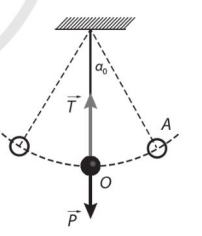
\includegraphics[width=0.3\linewidth]{../figs/D11-5-1}
	\end{center}
	Chọn gốc thế năng hấp dẫn tại vị trí cân bằng của vật nặng, áp dụng định luật bảo toàn cơ năng cho chuyển động của con lắc đơn ở môi trường không có lực cản:
	$$W_\text{O}=W_\text{A}\Leftrightarrow \dfrac{1}{2}mv^2_\text{max}=mg\ell\left(1-\cos\alpha_0\right)$$
	$$\Leftrightarrow v_\text{max}=\sqrt{2g\ell\left(1-\cos\alpha_0\right)}=\SI{1.78}{\meter/\second}$$
	Lực căng dây treo:
	$$T=mg+\dfrac{mv^2_\text{max}}{\ell}=\SI{6.23}{\newton}.$$
\end{enumerate}
}

\item \textbf{\textit{(1,0 điểm)}:}\\
Một con lắc lò xo đang dao động tắt dần với cơ năng ban đầu của nó là $\SI{10}{\joule}$, sau ba chu kì dao động biên độ của nó giảm $\SI{10}{\percent}$. Phần cơ năng chuyển hoá thành nhiệt sau khoảng thời gian đó bằng bao nhiêu?
\hideall{
Gọi $A$ là biên độ dao động ban đầu của vật nặng, cơ năng ban đầu của vật
$$W=\dfrac{1}{2}kA^2=\SI{10}{\joule}$$
Sau 3 chu kì dao động $A'=0,9A$
$$\Rightarrow W'=\dfrac{1}{2}kA'^2=0,81\cdot\dfrac{1}{2}kA^2=\SI{8.1}{\joule}$$
Phần cơ năng chuyển hoá thành nhiệt:
$$\Delta W=W-W'=\SI{1.9}{\joule}.$$
}

\item \textbf{\textit{(1,0 điểm)}:}\\
Một chiếc xe máy chạy trên một con đường lát gạch, cứ cách khoảng $\SI{4}{\meter}$ trên đường lại có một cái rãnh nhỏ. Chu kì dao động riêng của khung xe máy trên các lò xo giảm xóc là $\SI{0.5}{\second}$. Xe bị xóc mạnh nhất khi chuyển động với tốc độ bằng bao nhiêu?
\hideall{
	Xe bị xóc mạnh nhất khi chu kì ngoại lực kích thích bằng chu kì dao động riêng của khung xe $T=T_0=\SI{4}{\second}$.\\
	Tốc độ của xe khi xe xóc mạnh nhất:
	$$v=\dfrac{s}{T}=\SI{8}{\meter/\second}.$$
}
\end{enumerate}